\documentclass[a4paper,12pt]{article}
\usepackage{graphicx}
\graphicspath{ {./images/} }
\usepackage{wrapfig}
%\usepackage{fontspec}
\usepackage[utf8]{inputenc}
\usepackage[english]{babel}

\usepackage{hyperref}
\hypersetup{
  colorlinks=true,
  linkcolor=blue,
  filecolor=magenta,      
  urlcolor=cyan,
  pdftitle={RH Soil Sediment Sampling},
  bookmarks=true,
  %pdfpagemode=FullScreen,
}
%\urlstyle{same}

\title{A Soil Sediment Profile for Dar es Salaam}
\author{Ramani Huria}
\date{\today}

\begin{document}
\vbox{
  \centering
  
\includegraphics[width=3cm]{HOT_logo_with_text.png}
  \maketitle
}

\section{Executive Summary}
\label{executivesummary}
With the support of the World Bank in Tanzania, Ramani Huria (RH) and Jeremy Benn and Associates Consulting (JBA) partnered in October 2018 to develop a surface soil dataset for the greater Dar es Salaam region of Tanzania.  This was intended to support a geomorphological assessment taking into account soil characteristics for erosion and flood risk studies. 

A national-level soil profile had existed for Tanzania prior to this effort, but contained only a single sample from Dar es Salaam. This was not sufficient to analyse erosion potential across the city. The JBA team in consultation with Ramani Huria decided to use a 2km grid, which resulted in 731 sampling points being pre-established throughout the city.

A team of 10 field mappers and 4 office technicians---all Tanzanian youth participants in the Ramani Huria project---were trained in sample collection and analysis (sieving) respectively by JBA geomorphologist Matthew Hemsworth. A total of 643 points were sampled and sieved; 88 sites were inaccessible for one or another reason.

The 643 samples were analyzed by sieving each to separate the soil by particle size and weighing the resulting fractions. The resulting dataset, a geo-referenced set of soil profiles, is being published as open data.

\newpage
\section{Methodology}
\label{methodology}

\subsection{Field Sample Collection}
\label{fieldsamplecollection}
Two samples of 0.5kg of soil were collected in the field at---or if inaccessible, within 500m of---each of the pre-established sites. One sample was collected near the surface (after discarding 3cm of overlay, and the other at a depth between 7 and 15cm.

A set of data was recorded at each site using OpenDataKit's Android application ODK Collect. The team developed a form specific to this exercise. It included:
\begin{itemize}
  \item A GPS point
  \item Selection from a list of the Region, District, Ward, and Subward
  \item The ID number of the sample site (from the numbering of the 2km grid)
  \item A photograph before, during, and after the collection
  \item Information on accessibility
  \item A note if the weather was wet or dry
  \item Characteristics of the site (loose or consolidated sediment, low, medium, or high vegetation cover, rural or urban setting)
  \item A photo facing outward from the site in each cardinal direction
\end{itemize}

A copy of the field data collection form design in its original spreadsheet format is included in annex A (forms).

The team used a Kobo Toolbox instance as the back end (server) for the data collection. It was hosted on Digital Ocean, and set up using the procedure detailed \href{https://github.com/ivangayton/setup-scripts-various}{here}\footnote{\url https://github.com/ivangayton/setup-scripts-various. See the Readme and the file kobotoolbox\_secured\_server\_docker\_install}. The survey form was uploaded to this server, allowing all team members to download the black survey form, fill it out offline on their phones, and upload data back to the server. 

\newpage
\subsubsection{Materials}
Each field sampling team of two people carried the following equipemnt:
\begin{wrapfigure}{r}{0.25\textwidth} %this figure will be at the right
  \centering
  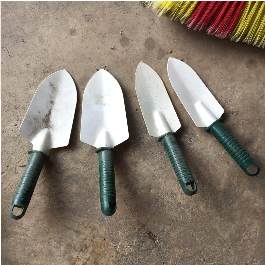
\includegraphics[width=0.25\textwidth]{trowels.png}
\end{wrapfigure}

\begin{itemize}
  \item Trowel or small shovel
  \item Plastic ``ziploc'' bags with ~1kg soil capacity
  \item Android phone pre-loaded with ODK Collect
  \item A separate maps and navigation application, maps.me, pre-loaded with the locations to be visited (the 2km grid)
  \item First aid kit
  \item Marker pens
  \item Permission letter for the sampling activity from the municipal authorities
  \item Tape measure
\end{itemize}

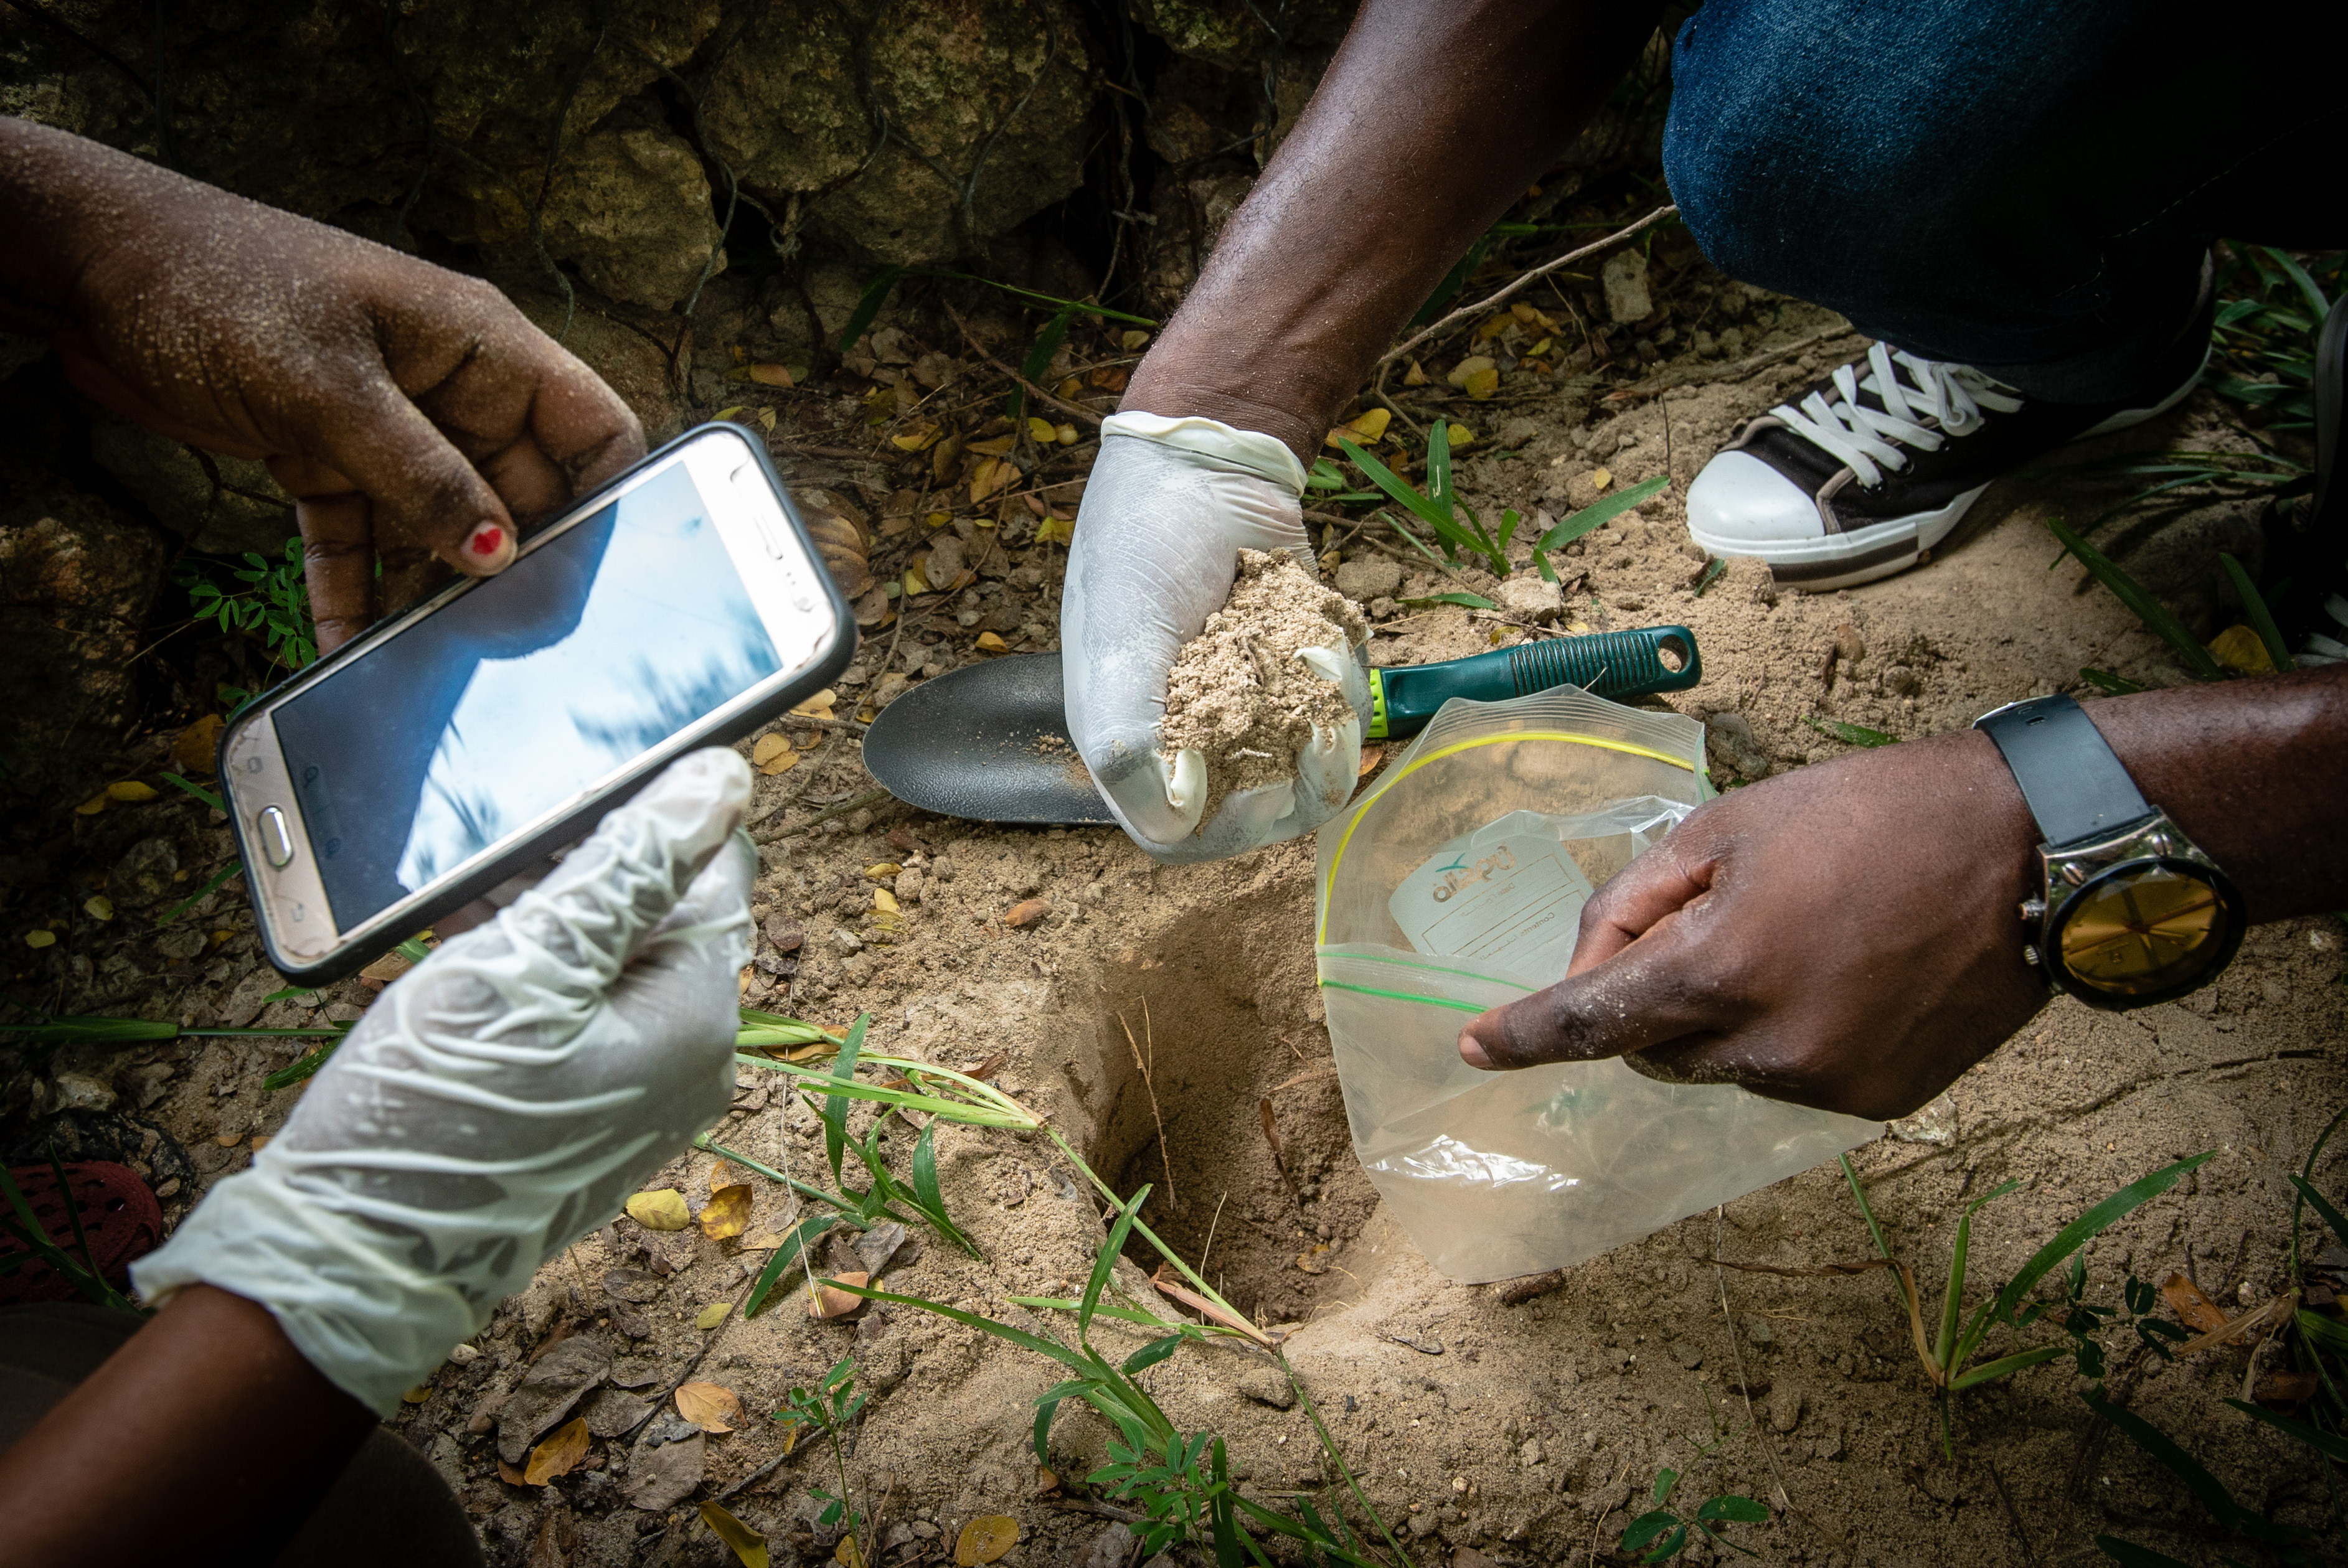
\includegraphics[width=\textwidth]{DSC05592.jpg}  

\subsubsection{Field Sampling Procedure}

Mappers used the following procedure as defined by JBA prior to commencement:
\begin{enumerate}
\item Navigate to the pre-defined sampling location.
\item Check the site is safe. If not, move on to the next site, and record the reason using ODK Collect.
\item If a sample cannot be taken (there may be a building or water body preventing access) the following procedure should be used: a suitable point within 500 metres of the defined sample location should be found by moving in a northerly direction. In some cases, points may simply not be accessible. In this case a reason should be recorded.
\item Once a suitable sample location has been identified use ODK Collect to record the relevant information by completing the survey form.
\item Use ODK Collect to take four photographs of the typical site surroundings (facing north, east, south, and west).
\item Begin taking the surface sediment sample using the following procedure:
\begin{enumerate}
\item Identify the area where you will take the sample. This should correspond
approximately to the sample point location, however it does not need to be exact.
\item Take a photograph of the ground before the sampling takes place
\item Remove the top layer of surface sediment using a pre-cleaned trowel or scoop (3 cm should be removed and discarded)
\item Collect one bag of sediment a depth between approximately 3cm - 7cm (TOP sample) and another from a depth approximately between 7cm and 15cm (BOTTOM sample). A tape measure should be used to measure the depths.
\item Place the collected sediment into plastic bags and tightly seal the them. If the bag appears at risk of breaking open the sample should be double bagged.
\item Each bag should be labelled with the unique site ID, either TOP or BOTTOM sample and the date using an indelible marker pen.
\item Move on to the next sample point.
\end{enumerate}
\end{enumerate}

\subsection{Laboratory Analysis}

The pair of samples---top and bottom---from each site was passed through a set of progressively finer-meshed sieves, resulting in nine separate fractions. Each fraction was weighed. The resulting measurements, which represent the proportion of each soil particle size at each site, were recorded.


\subsubsection{Materials}
%\begin{wrapfigure}{r}{0.2\textwidth}
%  \centering
%  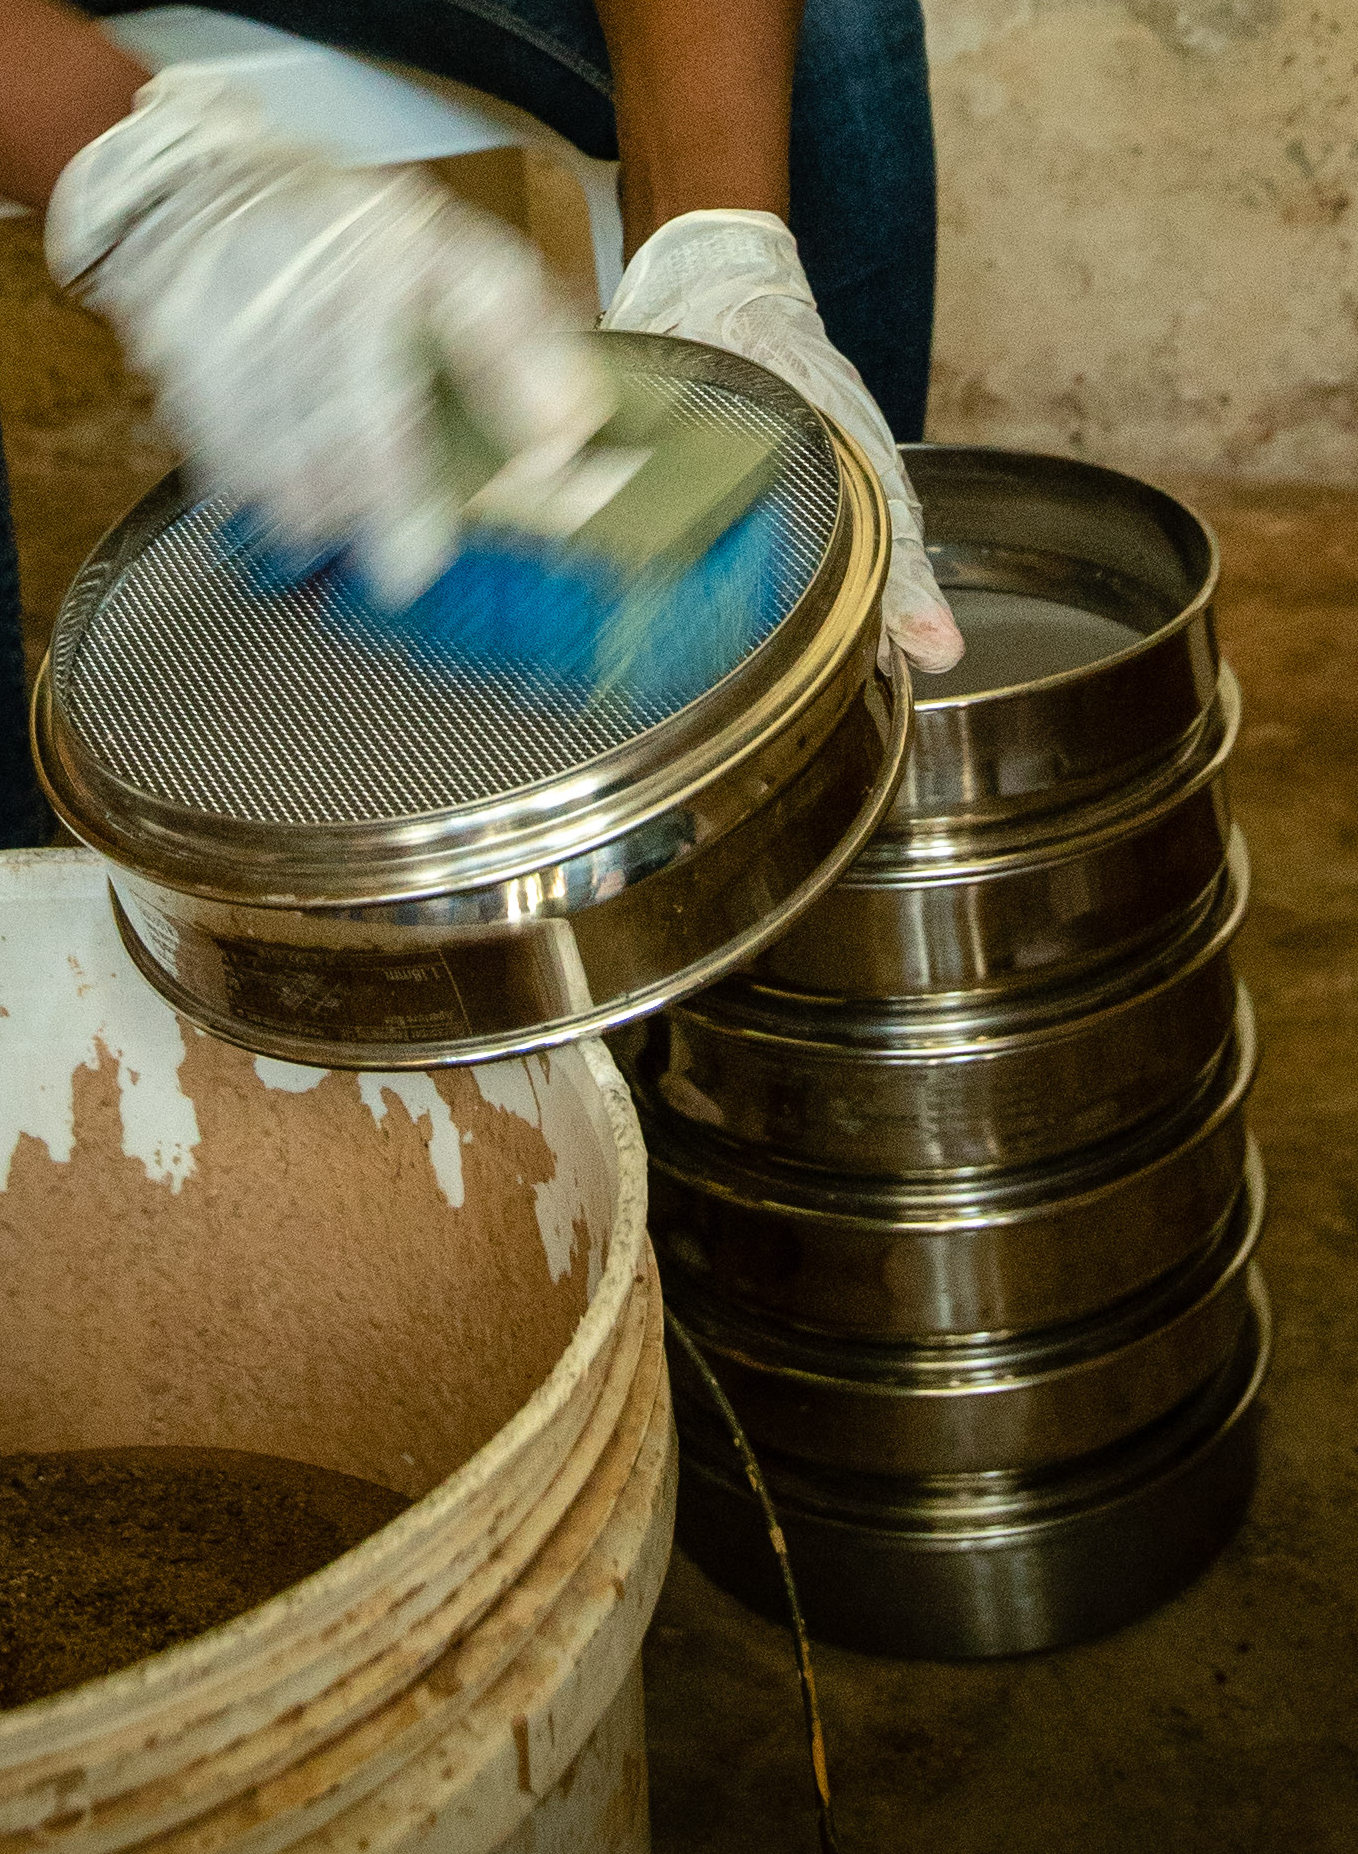
\includegraphics[width=0.18\textwidth]{DSC05543_cropped.jpg}
%\end{wrapfigure}
The following materials were used:

\begin{itemize}
  \item Set of metal sieves
  \item Scales
  \item Handwash station and gloves
  \item Brush, cloth, and towel for cleaning sieves
  \item Android phone with ODK Collect and sieving survey
\end{itemize}

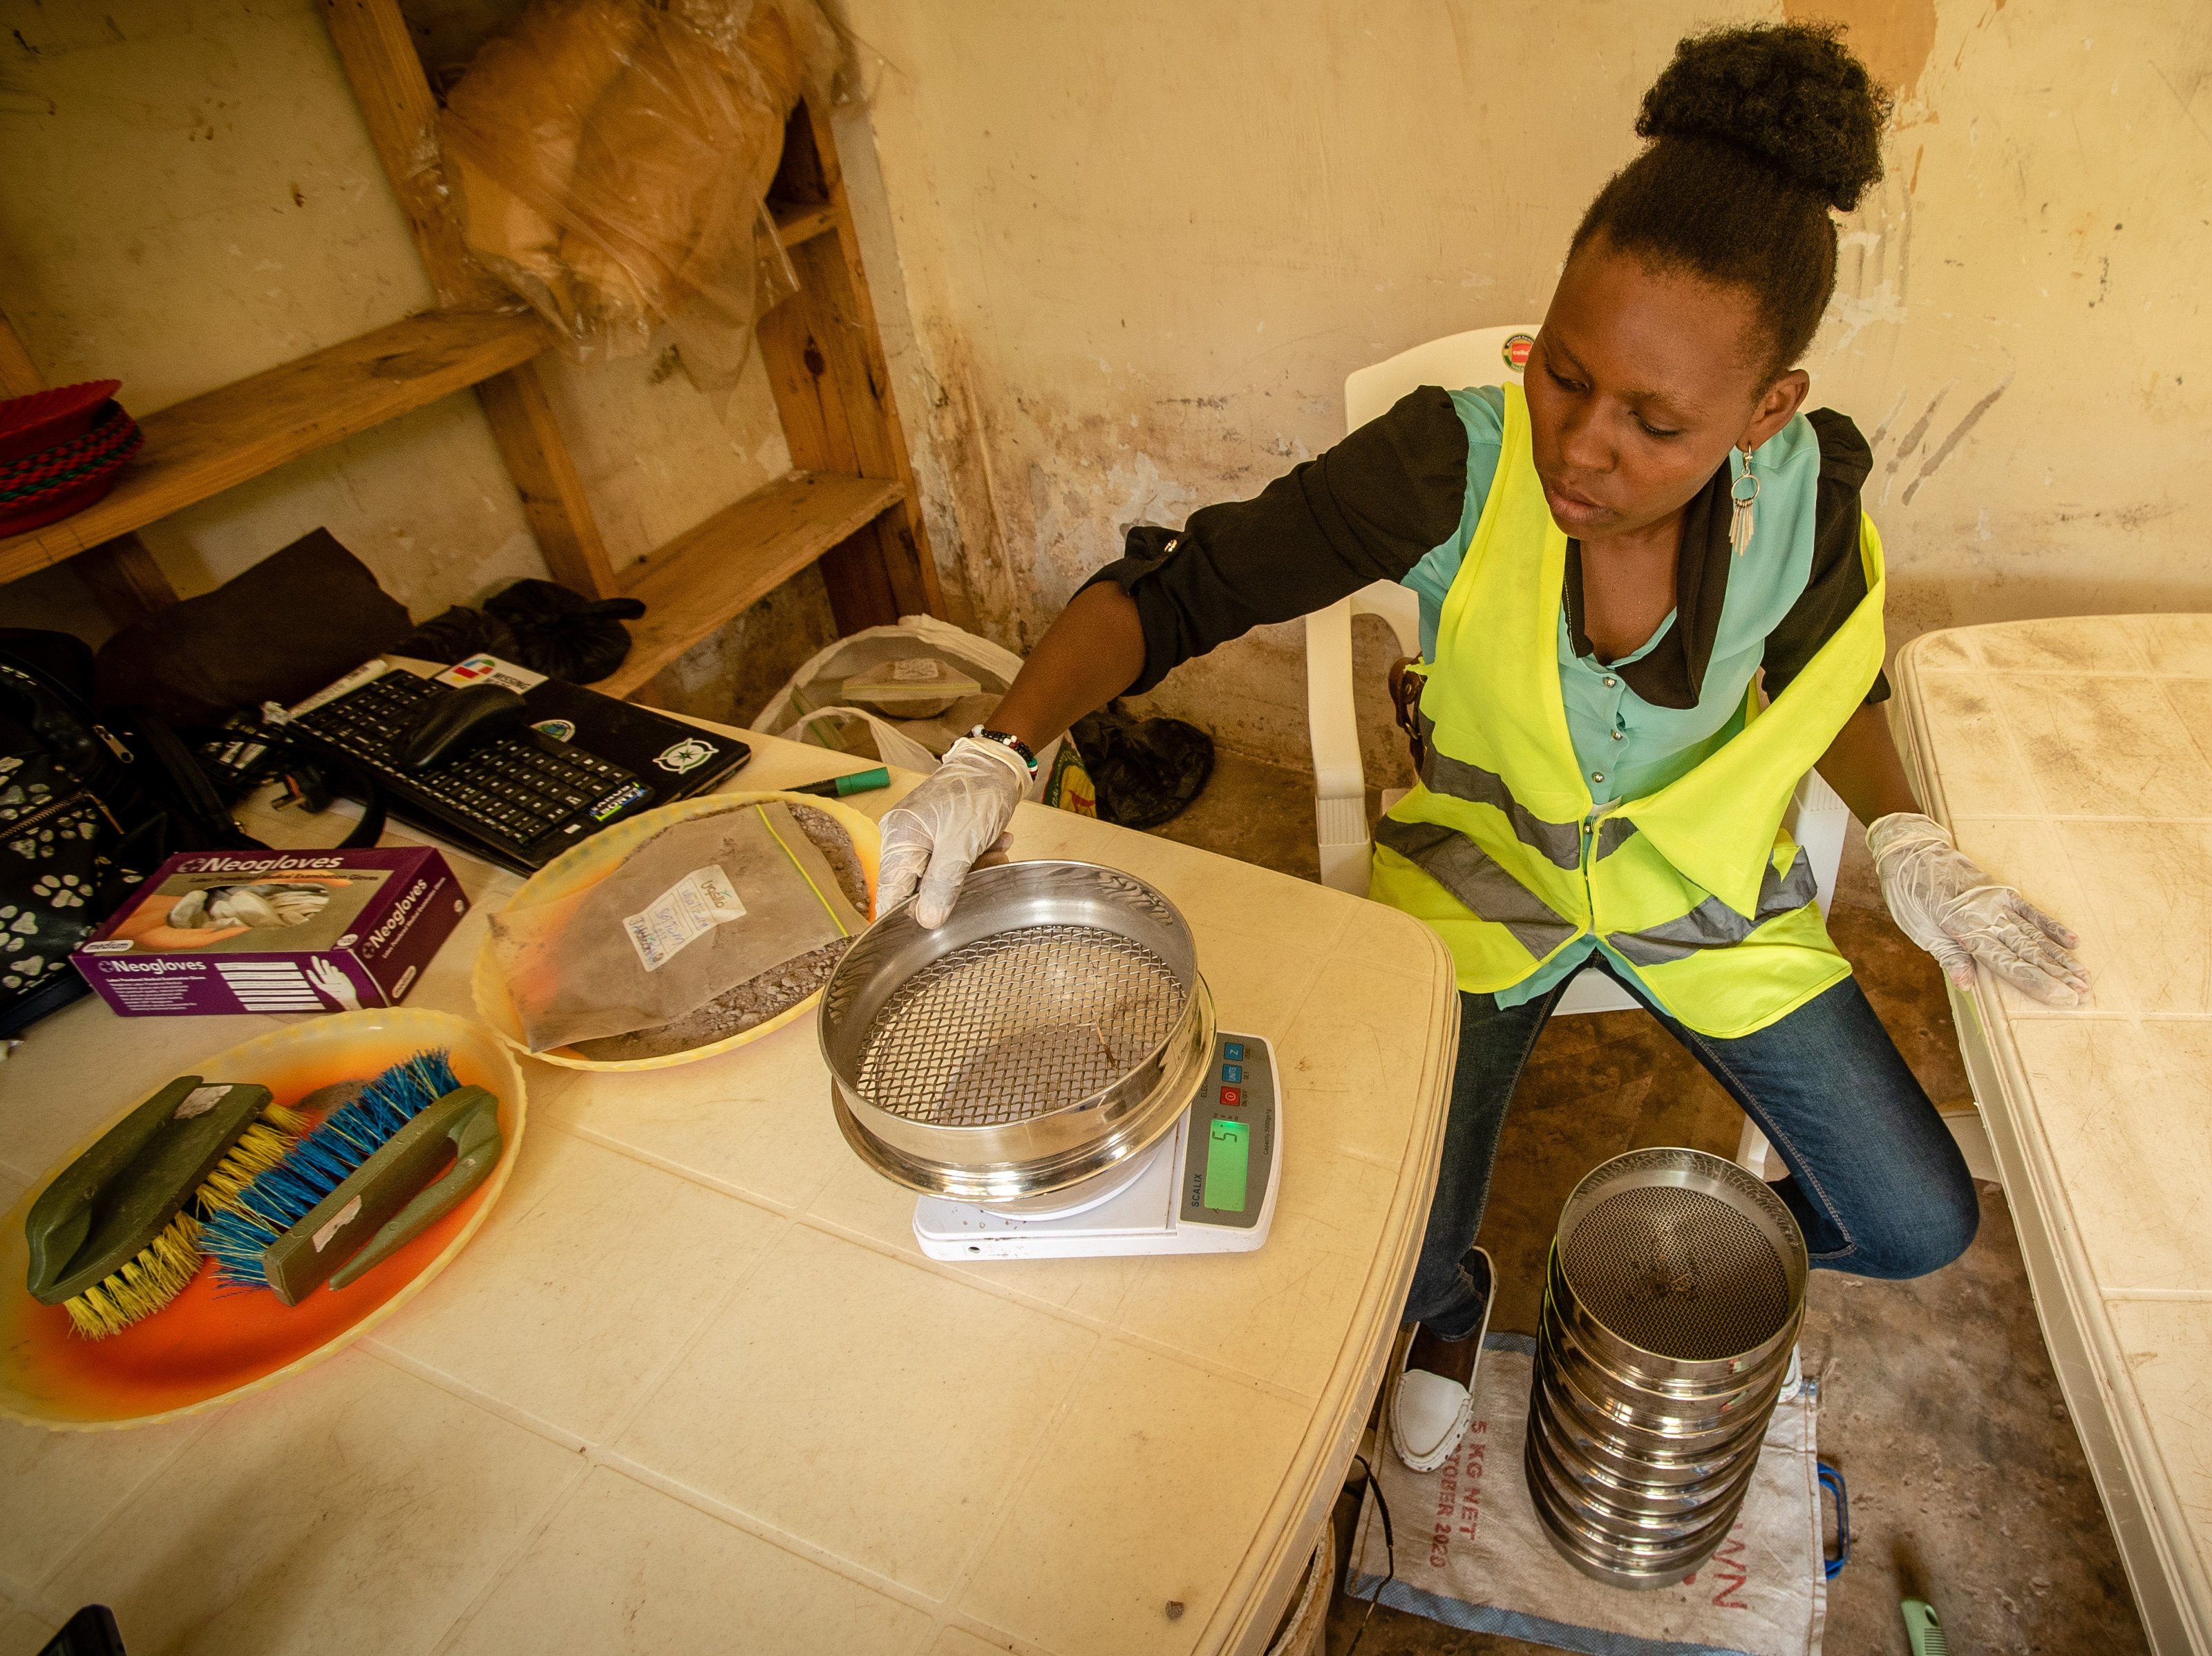
\includegraphics[ width=\textwidth]{DSC05570_cropped.jpg}

\subsubsection{Sieving and Data Entry}
The following procedure, specified by JBA, was used for the seiving.

\begin{enumerate}
  \item If samples are moist, they should be dried before analysis by being placed in the sun---though not exposed to wind---in a clean dry dish. 
  \item The following steps should be performed for both samples, beginning with the TOP sample.
  \item Weigh about 500g of sediment from the bag into a weighing dish.
  \item If soil particles are lumped or conglomerated, crush the lumped particles until they become loose.
  \item Determine the mass (weight in grams) of each sample before sieving.
  \item Prepare a stack of sieves. Those with larger opening sizes are placed above the ones with smaller opening sizes. The lowest on the stack is a simple pan which retains the soil that passes through the finest sieve.
  \item Make sure all sieves are clean---if any soil particles are stuck in the openings poke them out using the brush.
  \item Weigh all empty sieves and the pan separately. Record the results in ODK Collect.
  \item Pour the sediment into the stack of sieves from the top and place the cover on top. Shake the sieves carefully so the sediment filters through---this may need to be done for 3 to 5 minutes.
  \item Stop shaking and measure the mass of each sieve + retained soil. Record the results in ODK Collect.
\end{enumerate}

Initially a Google Sheets spreadsheet was created to store the results. Each site (set of two samples) had a single tab on the spreadsheet, with the tab named for the site ID number. The sievers would use the $move or copy sheet$ function in Google Sheets to create a new tab, rename that tab to the sample ID, and fill in the data. Calculations and checks were automatic. However, the RH team did not do well with this (see discussion in the \hyperlink{lessonslearned}{lessons learned} section). Therefore an ODK form was created to record the results, which eventually made for a more effective process. 

\newpage 
\section{Results and Analysis}
\label{resultsandanalysis}
The team sampled 643 sites, top and bottom (1286 soil samples in total). The primary result is a table of masses representing the proportion of soil.

This data is primarily intended for use with erosion modeling. For users not equipped with erosion modeling skills and toolkits, and for sharing the results with the public, a visual map has been prepared that gives a good first impression of the characteristics of the soil.


\begin{figure}[h]
  \caption{The bars of the histogram---upper for the top samples and lower for the bottom samples---represent the proportion of soil of each particle size.}
  \centering
  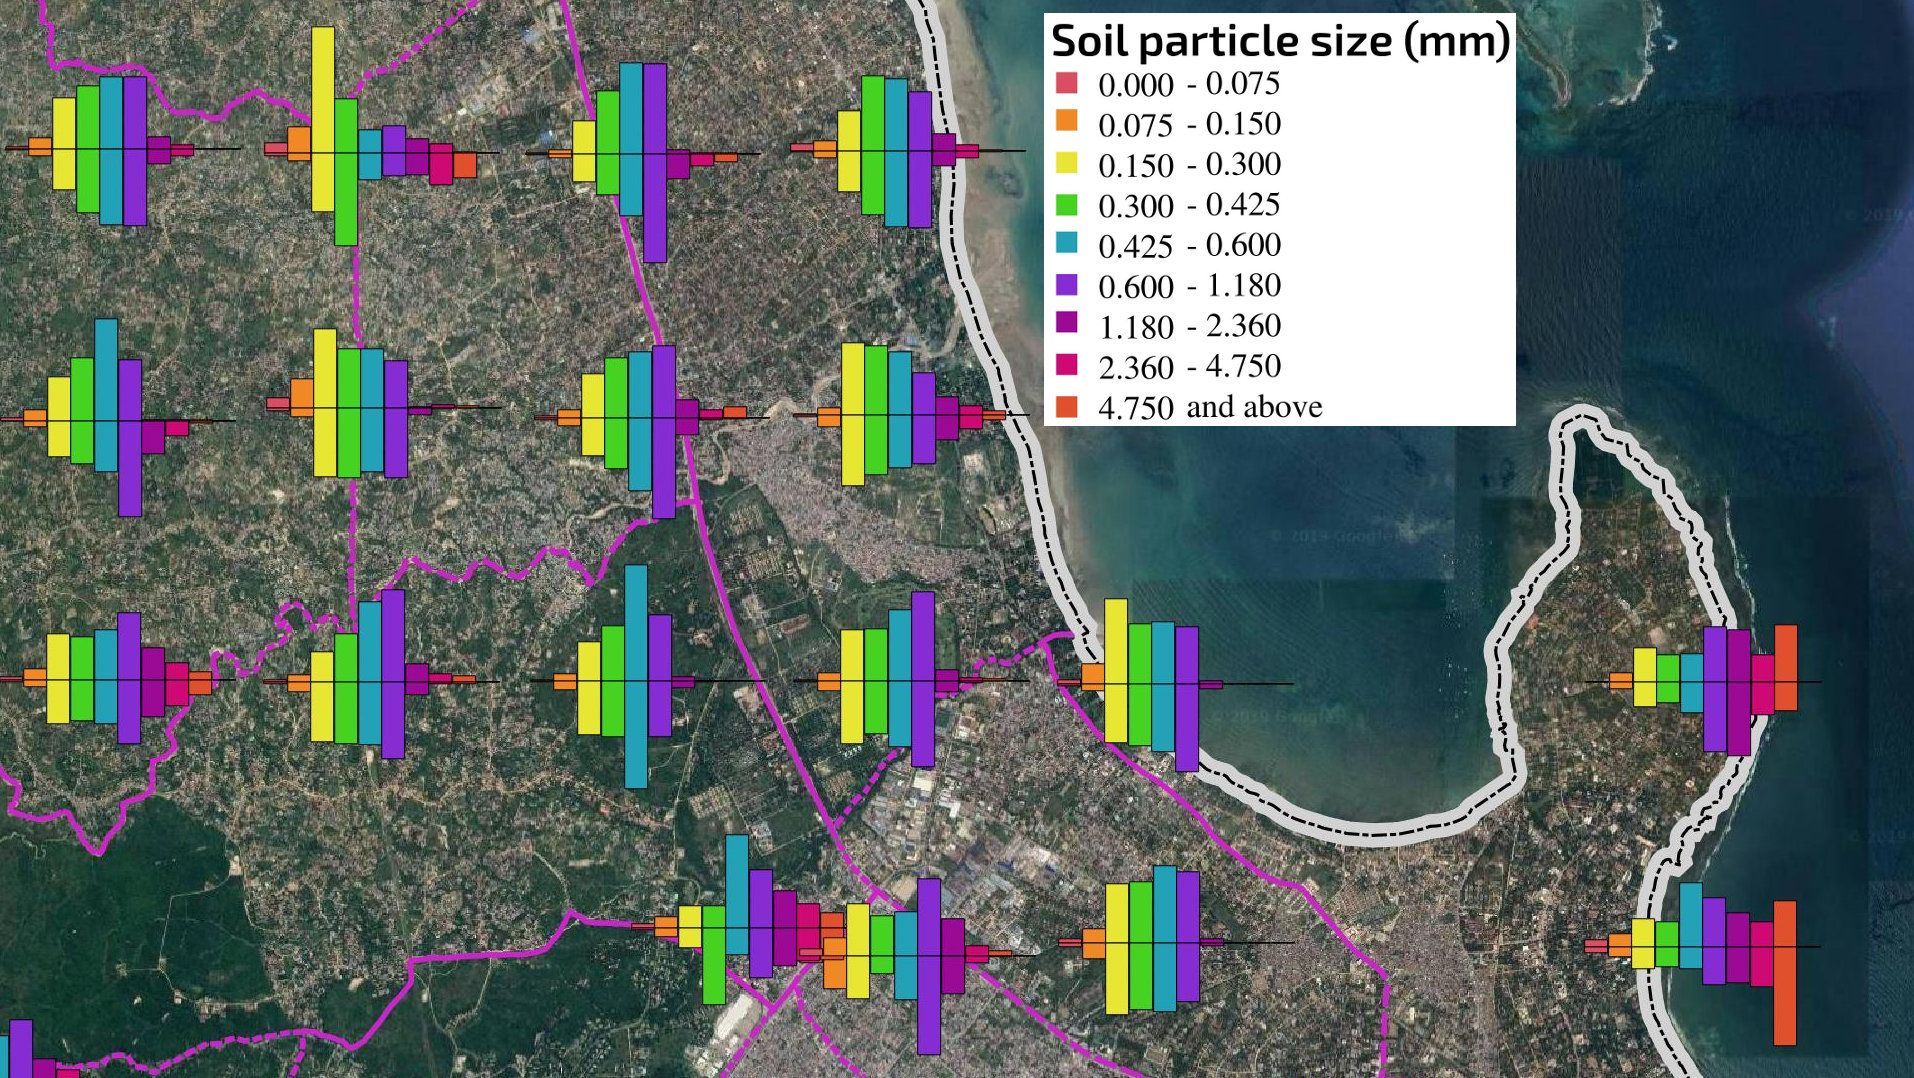
\includegraphics[width=1.1\textwidth]{soil_map_detail_peninsula_with_legend}
\end{figure}



\section{Lessons Learned}
\label{lessonslearned}

\hypertarget{lessonslearned}{}

\begin{itemize}
  \item RH youth can deliver good quality data, but it's important to have pretty frequent check-ins to ensure things don't drift or degrade.
  \item It's critical to design the tools really, really carefully. We fell down a bit on data entry, in part because we didn't invest enough in making sure the system was robust and simple.
  \item When you need 18 precise measurements (9 top and 9 bottom portions, not to mention the initial total masses and the empty sieve masses) for a single site/sample to be correct, what looks like a low error rate upon a cursory inspection is actually quite a high one! A single mistake in 100 measurements makes 1/5 of the sites invalid.
  \item In the end, the data was actually really good. It just took a lot more effort than expected to get there.
\end{itemize}
\end{document}

